\documentclass{sosg-informe}

\graphicspath{{../../geodatos/estudios/tormentas/figuras/}{../../geodatos/estudios/idf/figuras/}}

\title{Tormentas sintéticas y curvas IDF provisionales\\para la alerta de inundación por lluvia\\en Santa Cruz y San Cristóbal (Galápagos)}
\titulocorto{Tormentas sintéticas y curvas IDF}
\numero{2026-02}
\estado{Borrador para discusión}
\titulocita{Tormentas sintéticas y curvas IDF provisionales para la alerta de inundación por lluvia en Santa Cruz y San Cristóbal (Galápagos)}
\relacionados{Issues \issue{19}, \issue{24}, \issue{26} y \issue{30} · repositorio mayait/sosgalapagos-datos}
\date{4 de noviembre de 2026}

\begin{document}
\maketitle

\begin{abstract}
La tormenta del 30 de octubre de 2026 inundó La Cascada (Puerto Ayora) con 61--66~mm en una hora y hasta 240~mm en el día. La regla de alerta vigente (v0.2) da el nivel \alto{} con 30~mm en 1~h, 60~mm en 3~h o 100~mm en 24~h, pero nunca se había evaluado frente a un conjunto amplio de eventos. Se generaron 500 tormentas sintéticas por isla, con formas convectivas, orográficas y uniformes, de 1 a 24~h. Cada una se propagó con un modelo hidrodinámico 2D de inercia local sobre un DSM de 30~m, validado contra las corridas originales con diferencias de 1~cm y 2~min. Para poner esas tormentas en una escala de años se construyeron curvas intensidad-duración-frecuencia (IDF) provisionales. La lluvia de un día sale de los máximos anuales de la Fundación Charles Darwin (61 y 31 años, ajuste de Gumbel). El reparto en horas sale del reanálisis GAR (WRF de 2~km, 1980--2025), y se contrastó con lluvia medida cada 5 minutos. La regla v0.2 avisa a tiempo entre el 87\,\% y el 100\,\% de las inundaciones modeladas, con 25~min a 2~h de anticipación. A cambio, daría \alto{} aproximadamente una vez cada 1,6--1,9 años por zona: cerca de una falsa alarma cada dos años. Las zonas que más se inundarían son Barrio Frío (${\approx}\,1$ vez cada 8 años) y La Cascada (${\approx}\,1$ vez cada 12 años). El 30-oct corresponde a una lluvia de unos 15 a 55 años. Elevar los umbrales un 10\,\% habría retrasado tres horas el único aviso real disponible, así que los resultados no justifican subirlos mientras no haya validación histórica. Todas las cifras son estimaciones de modelo, sin validar con inundaciones históricas.
\palabrasclave{alerta temprana; inundación pluvial; modelo 2D de inercia local; tormentas sintéticas; curvas IDF; periodo de retorno; Galápagos.}
\end{abstract}

\begin{aviso}
Este informe presenta \textbf{modelos propios, no datos oficiales}. Las curvas IDF son un orden de magnitud y no deben usarse para diseñar obras. Las frecuencias de inundación no están validadas con eventos históricos. La referencia oficial para intensidades sería el estudio del \citet{inamhi2015}, que aún no se ha obtenido. El análisis lo preparó un equipo asistido por agentes de inteligencia artificial, sin visitas de campo ni revisión profesional externa, y no expresa una posición institucional de la USFQ. Usa lluvia medida del IERSE (CC BY-NC-ND 4.0) y de la FCD (CC BY-NC-SA); los productos derivados de esas series quedan sujetos a sus licencias y al permiso de sus titulares.
\end{aviso}

% =====================================================================
\section{Introducción}

Santa Cruz y San Cristóbal no tienen ríos permanentes. Sus inundaciones son repentinas: el agua de lluvia baja por quebradas secas (\enquote{cañadas}) y se acumula en barrios construidos sobre depresiones del terreno o en la desembocadura de esos cauces. El 30 de octubre de 2026, un núcleo convectivo sobre la parte alta de Santa Cruz dejó entre 61 y 66~mm/h en las estaciones de la red IERSE-WSN y 117--131~mm en tres horas. Por la noche inundó el sector de La Cascada, en Puerto Ayora.

SOS Galápagos opera desde 2026 una alerta por lluvia basada en los pluviómetros disponibles de IERSE, INAMHI y USFQ GSC. Su regla v0.2 da el nivel \alto{} cuando el máximo ponderado de las estaciones de una zona supera 30~mm en 1~h, 60~mm en 3~h o 100~mm en 24~h. Esa regla se fijó con un solo evento observado. No se sabía cuántas inundaciones avisaría, con cuánta anticipación ni cada cuánto daría falsas alarmas.

Este trabajo responde esas preguntas con dos herramientas. Para la primera se usa la idea de los gemelos digitales de crecidas, por ejemplo PGTEC (UPV, 2026), que combina los modelos TETIS e HIDRIS: se generan muchas tormentas plausibles, se mueven y escalan sobre el terreno, y se observa qué marca cada pluviómetro cuando algo se inunda abajo (secciones~\ref{sec:generador}--\ref{sec:criterios}). La segunda son curvas IDF provisionales, que permiten traducir cada tormenta y cada umbral a un periodo de retorno y a una frecuencia anual (secciones~\ref{sec:idf}--\ref{sec:frecuencia}).

% =====================================================================
\section{Área de estudio y datos}

\subsection{Zonas de impacto}
Se evaluaron seis zonas con antecedentes o sospecha de inundación:
\begin{itemize}
  \item en Santa Cruz: La Cascada, Tomás de Berlanga y Bellavista;
  \item en San Cristóbal: la desembocadura de Barrio Frío, El Manzanillo y El Progreso.
\end{itemize}
Cada zona se representa con un punto clave en la celda de 30~m del modelo, y tiene asignadas las estaciones de la regla v0.2 con su peso.

\subsection{Lluvia medida}
\begin{itemize}
  \item \textbf{Red IERSE-WSN (Universidad del Azuay):} registros de 5--10~min desde abril de 2026, en Los Guayabillos (178~m), Santa Rosa (422~m), Cerro Crocker y otros puntos de Santa Cruz.
  \item \textbf{INAMHI:} estaciones de Puerto Ayora y Puerto Baquerizo Moreno.
  \item \textbf{USFQ GSC:} El Junco, Cerro Alto y El Mirador, en San Cristóbal.
  \item \textbf{Fundación Charles Darwin (FCD):} lluvia diaria de lectura manual en Puerto Ayora (1965--2025, 61 años válidos) y Bellavista (1988--2018, 31 años). Se usan solo los años con al menos 330 días.
\end{itemize}

\subsection{Reanálisis y terreno}
\begin{itemize}
  \item \textbf{GAR} (\emph{Galápagos Archipelago Refined analysis}; \citealp{schmidt2025}): WRF 4.3.3 a 2~km, forzado con ERA5, 1980--2025, con lluvia horaria (CC BY 4.0). Es \emph{lluvia modelada}.
  \item \textbf{Terreno:} el DSM Copernicus GLO-30 \citep{esa2021}. Incluye techos y vegetación, y tiene un sesgo vertical de $-2$ a $-3$~m frente al IGM.
\end{itemize}

% =====================================================================
\section{Métodos}

\subsection{Generador de tormentas sintéticas}\label{sec:generador}
Se generaron 500 tormentas por isla con semillas fijas (20261030 para Santa Cruz y 20261031 para San Cristóbal).
\begin{itemize}
  \item \textbf{Forma en el espacio:}
  \begin{itemize}
    \item 55\,\%: núcleos convectivos gaussianos de radio 1,5--6~km, que pueden desplazarse a 0--14~km/h. El 65\,\% de ellos se centra en la parte alta.
    \item 25\,\%: tormentas orográficas, con lluvia creciente con la cota.
    \item 20\,\%: tormentas uniformes.
  \end{itemize}
  \item \textbf{Forma en el tiempo:} sigue una distribución beta con la moda entre el 20 y el 80\,\% de una duración $d$ de 1 a 24~h.
  \item \textbf{Lámina máxima en el núcleo:} está acotada por
\end{itemize}
\begin{equation}
  D_{\max}(d) = 90\, d^{\,0,42}\ \text{mm}, \qquad d \text{ en horas},
\end{equation}
que da 90~mm en 1~h, 141~mm en 3~h y 340~mm en 24~h. Es del orden del 30-oct, un evento de decenas de años. Dos parámetros, inciertos, se muestrean en lugar de fijarse:
\begin{itemize}
  \item la humedad antecedente $P_{5d}$, entre 0 y 100~mm;
  \item la pérdida constante del suelo $F$: 15--35~mm/h en Santa Cruz, según el barrido de calibración del 30-oct, y 5--35~mm/h en San Cristóbal, donde no está calibrada.
\end{itemize}
La pérdida inicial disminuye con la humedad antecedente: $\mathit{IL} = \mathit{IL}_0 \cdot \operatorname{clip}(1,4 - P_{5d}/60;\ 0,2;\ 1,4)$. La figura~\ref{fig:generador} muestra seis tormentas del conjunto.

\begin{figure}[t]
  \centering
  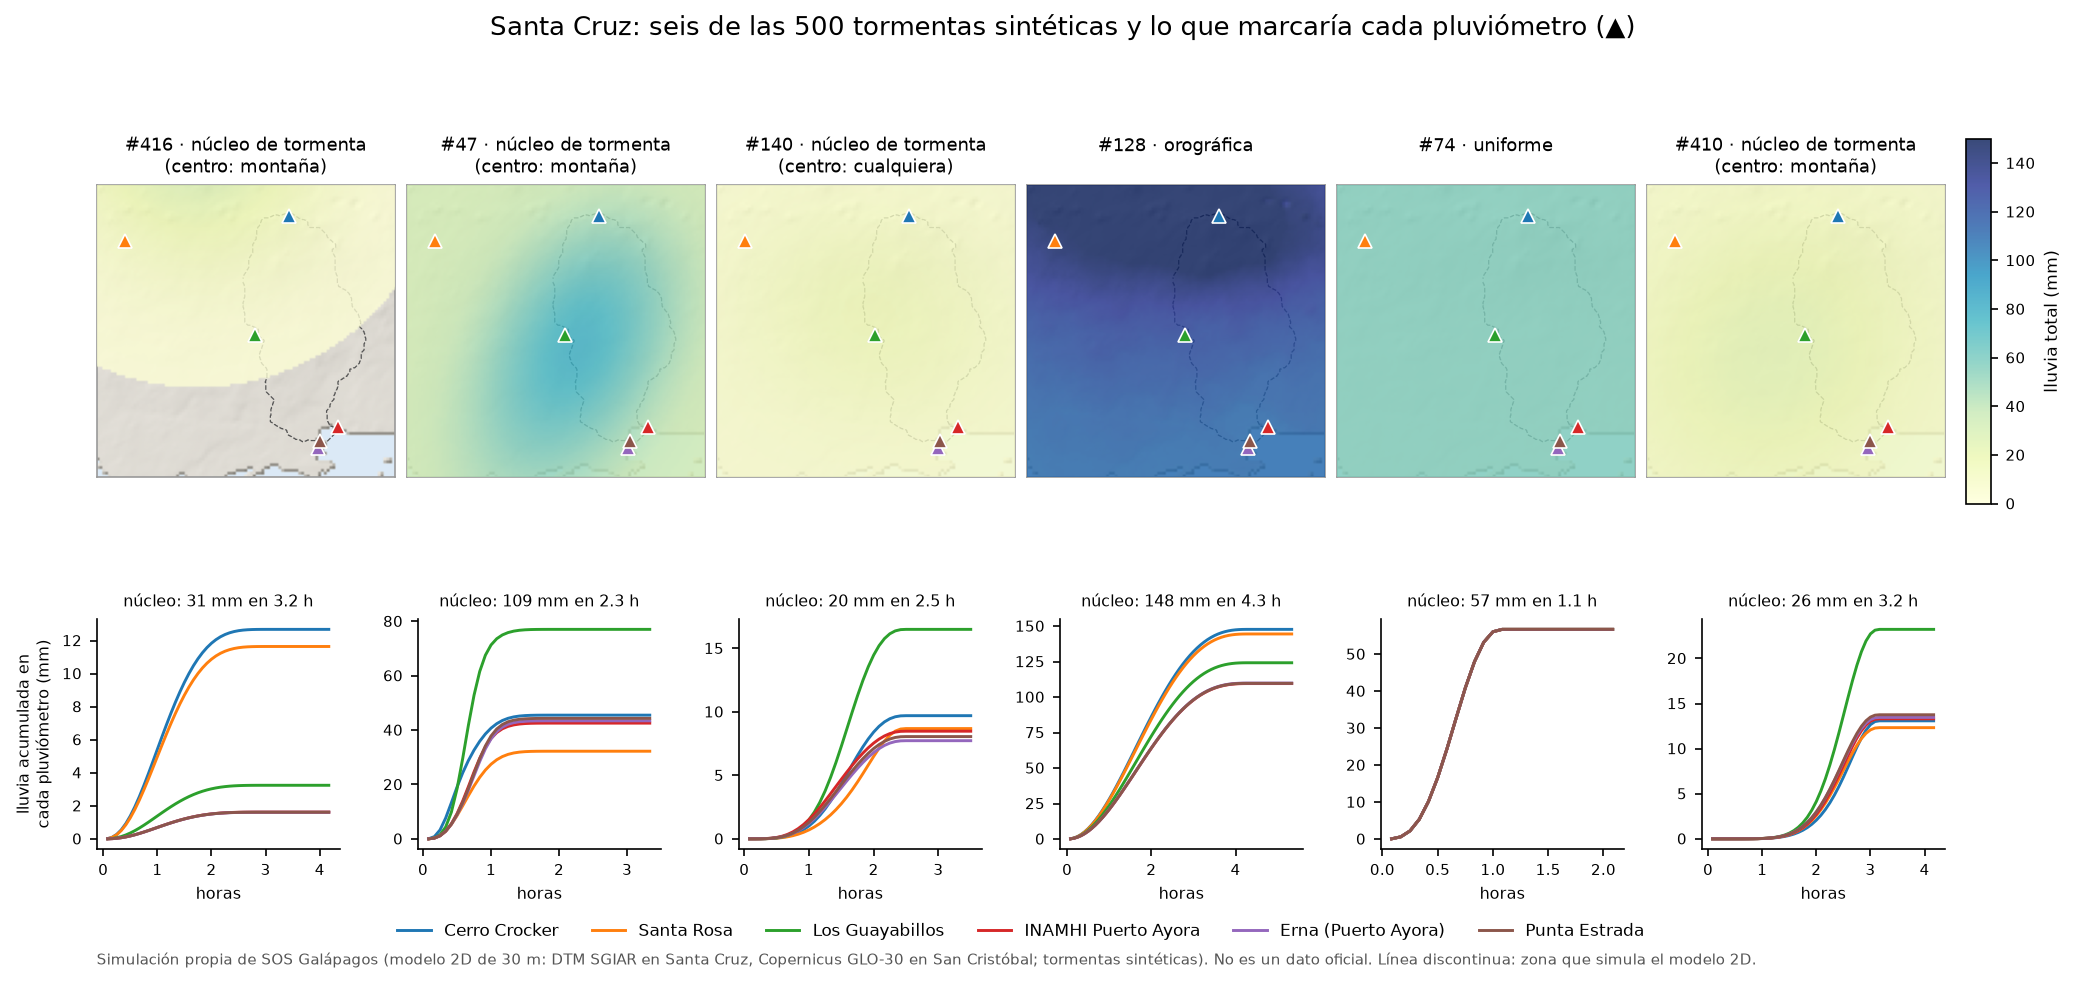
\includegraphics[width=\linewidth]{generador_santa-cruz.png}
  \caption{Seis de las 500 tormentas sintéticas de Santa Cruz: núcleos convectivos, orográfica y uniforme. Arriba, la lluvia total de cada una, con los pluviómetros (\(\blacktriangle\)); abajo, la lluvia acumulada que marcaría cada pluviómetro.}
  \label{fig:generador}
\end{figure}

\subsection{Modelo hidrodinámico 2D}
Cada tormenta se propagó con un esquema de inercia local \citep[LISFLOOD-FP \enquote{acc};][]{bates2010} sobre una malla regular de 30~m. Se aplicó la ponderación $\theta = 0,8$ de \citet{dealmeida2012}. El caudal unitario entre celdas se actualiza como
\begin{equation}
  q^{\,t+\Delta t} = \frac{\theta\, q^{\,t} + \tfrac{1}{2}(1-\theta)\left(q^{\,t}_{-} + q^{\,t}_{+}\right) - g\, h_f\, \Delta t\, \dfrac{\partial (h+z)}{\partial x}}{1 + g\, \Delta t\, n^2\, \lvert q^{\,t}\rvert \,/\, h_f^{7/3}},
\end{equation}
donde:
\begin{itemize}
  \item $h_f$ es la profundidad de flujo entre celdas;
  \item $z$ es la cota;
  \item $n$ es el coeficiente de Manning;
  \item $\Delta t$ se adapta con un número de Courant $\alpha = 0,7$.
\end{itemize}

El esquema de los modelos originales de cada isla (scripts 24 y 25 del repositorio) se reescribió en una sola función compilada con numba. Las condiciones de borde son distintas en cada isla:
\begin{itemize}
  \item Santa Cruz: mar a nivel fijo y contorno de tierra cerrado;
  \item San Cristóbal: limitador de Froude 1, y mar y bordes absorbentes.
\end{itemize}
Una tormenta tarda 9~s en Santa Cruz y 3~s en San Cristóbal, así que el lote completo se corre en unos 18~min con 9 procesos.

\subsection{Criterios de inundación y de aviso}\label{sec:criterios}
Una zona se considera \emph{inundada} si el calado máximo en su punto clave alcanza 0,3~m. Un aviso es \emph{a tiempo} si la regla da \alto{} al menos 15~min antes de que el agua llegue a ese calado. Cada pluviómetro \enquote{mide} la lluvia del campo sintético en su posición, sin error de medida ni cortes de transmisión.

La capacidad de cada estación para anticipar la inundación se midió con el área bajo la curva ROC \citep[AUC;][]{fawcett2006}. El predictor es la lluvia acumulada en las 3~h previas a la llegada del agua: 0,5 equivale a no discriminar y 1 a hacerlo perfectamente. El mismo criterio se aplicó en cada celda del dominio para buscar el mejor sitio para un pluviómetro nuevo.

\subsection{Curvas IDF provisionales}\label{sec:idf}
Los máximos anuales de lluvia diaria de la FCD se ajustaron por máxima verosimilitud a una distribución de Gumbel (central) y a una GEV \citep[sensibilidad;][]{coles2001}. Los intervalos de confianza del 90\,\% salen de 1000 remuestreos de los años \citep[\emph{bootstrap};][]{efron1993}. Para una duración $d$ y un periodo de retorno $T$, la lámina se obtiene con el método del índice \citep{hosking1997}:
\begin{equation}
  R(d,T) = r(d)\; x_{1d}(T), \qquad x_{1d}(T) = \mu - \beta \ln\!\left[-\ln\!\left(1 - \frac{1}{T}\right)\right],
\end{equation}
donde $\mu$ y $\beta$ son los parámetros de Gumbel de la estación de la FCD de referencia:
\begin{itemize}
  \item Puerto Ayora: $\mu = 47,4$~mm, $\beta = 37,9$~mm;
  \item Bellavista: $\mu = 60,1$~mm, $\beta = 38,0$~mm.
\end{itemize}

La razón $r(d)$ es la media de los máximos anuales de $d$ horas en GAR dividida por la media de los máximos anuales de un día, para $d = 1, 2, 3, 6$ y 12~h. Descargar GAR horario completo exige unos 30~GB, así que solo se leyeron por rangos de bytes los \textbf{cinco días más lluviosos de cada año en cada isla}: 385 días en total. Las ventanas horarias se cuentan dentro del día UTC, que va de 18:00 a 18:00 en hora de Galápagos.

Para 24~h móviles se usa $r(24) = 1,13$, el factor de \citet{weiss1964} para pasar de un intervalo fijo a uno móvil. Las sumas horarias de GAR reproducen exactamente su lluvia diaria.

Cada pluviómetro toma la curva diaria de la estación de la FCD más parecida en altura: Puerto Ayora por debajo de 100~m y Bellavista por encima. No se aplica el gradiente de altura de GAR porque no está validado: en la celda de Santa Rosa da 1,8 veces la lluvia medida en Bellavista. San Cristóbal no tiene una serie diaria larga disponible, así que toma prestada la curva de Santa Cruz a la misma altura. Sus razones horarias sí son las de GAR en sus propios puntos.

\subsection{Periodo de retorno de una tormenta y frecuencia anual}\label{sec:frecuencia}
Para cada tormenta y cada estación de la regla de una zona se calcula $T(R_d)$ para $d = 1, 3, 6$ y 24~h. El periodo de retorno de la tormenta en la zona es el máximo de esos valores. La probabilidad de inundarse se ajustó con una regresión logística sobre $\ln T$:
\begin{equation}
  P(\text{inund.} \mid T) = \frac{1}{1 + \exp\left(-a - b \ln T\right)}.
\end{equation}
La probabilidad anual se obtiene integrando esa curva sobre la distribución de los máximos anuales, con $u \sim \mathcal{U}(0;\,0,9995)$ y $T = 1/(1-u)$:
\begin{equation}
  p_{\text{anual}} = \int P\bigl(\text{inund.} \mid T(u)\bigr)\, \mathrm{d}u .
\end{equation}
Para la frecuencia del nivel \alto{} se toma el periodo $T_{\text{alto}}$, el mínimo entre estaciones y duraciones de $T(\text{umbral}/\text{peso})$. Se convierte en eventos por año con la relación de \citet{langbein1949}, $\lambda = -\ln(1 - 1/T)$. Las falsas alarmas por año se aproximan como $\lambda_{\text{alto}} - \lambda_{\text{inund.}}$.

Los mapas por periodo de retorno muestran, en cada celda, la fracción de tormentas con calado $\geq 0,3$~m dentro de tres bandas: 2--10, 10--50 y $\geq 50$ años. El mapa anual combina siete bandas, cada una ponderada por $1/T_{\inf} - 1/T_{\sup}$.

% =====================================================================
\section{Resultados}

\subsection{Validación del motor}
El motor reescrito reproduce las corridas originales (tabla~\ref{tab:validacion}). En La Cascada, el calado máximo difiere en 1~cm y las horas de llegada y de máximo en 1--2~min. En San Cristóbal los puntos del modelo original coinciden al centímetro.

\begin{table}[ht]
  \centering\small
  \caption{Validación del motor 2D reescrito frente al modelo original con la lluvia medida del 30-oct-2026 (Santa Cruz, La Cascada). Horas locales (UTC$-6$).}
  \label{tab:validacion}
  \begin{tabular}{lcc}
    \toprule
    Magnitud & Motor nuevo & Modelo original \\
    \midrule
    Calado máximo & 1,85~m & 1,84~m \\
    Llegada de 0,1~m & 20:55 & 20:53 \\
    Hora del máximo & 22:25 & 22:24 \\
    \bottomrule
  \end{tabular}
\end{table}

\subsection{Desempeño de la regla v0.2}
Con las 500 tormentas, la regla v0.2 avisa a tiempo el 87--100\,\% de las inundaciones modeladas (tabla~\ref{tab:v02}). La anticipación típica va de 2~h en La Cascada a 25~min en Barrio Frío. Allí la cuenca es corta y el agua llega poco después del chubasco. La proporción de tormentas sin inundación que igual dan \alto{} es alta, del 37\,\% al 59\,\%. Esa proporción es del conjunto sintético, que está cargado a propósito hacia tormentas fuertes. \textbf{No es una frecuencia anual de falsas alarmas}; esa se estima en la sección~\ref{sec:res-frecuencia}. La figura~\ref{fig:frecuencia} muestra dónde se junta el agua con más frecuencia dentro del conjunto.

\begin{table}[ht]
  \centering\small
  \caption{Regla v0.2 aplicada a 500 tormentas sintéticas por isla. \enquote{Falsas alarmas} = tormentas sin inundación (calado $< 0,3$~m) que dan \alto.}
  \label{tab:v02}
  \begin{tabularx}{\linewidth}{>{\raggedright\arraybackslash}Xlcccc}
    \toprule
    Zona & Isla & \makecell{Tormentas\\que inundan} & \makecell{Avisadas\\a tiempo} & \makecell{Falsas alarmas\\(conjunto)} & \makecell{Aviso\\típico} \\
    \midrule
    La Cascada & Santa Cruz & 141 & 98\,\% & 37\,\% & 2~h \\
    Tomás de Berlanga & Santa Cruz & 50 & 100\,\% & 49\,\% & 70~min \\
    Bellavista & Santa Cruz & 127 & 95\,\% & 47\,\% & 50~min \\
    Barrio Frío (desembocadura) & San Cristóbal & 153 & 87\,\% & 49\,\% & 25~min \\
    El Manzanillo & San Cristóbal & 74 & 96\,\% & 59\,\% & 50~min \\
    El Progreso & San Cristóbal & 68 & 93\,\% & 59\,\% & 30~min \\
    \bottomrule
  \end{tabularx}
\end{table}

\begin{figure}[t]
  \centering
  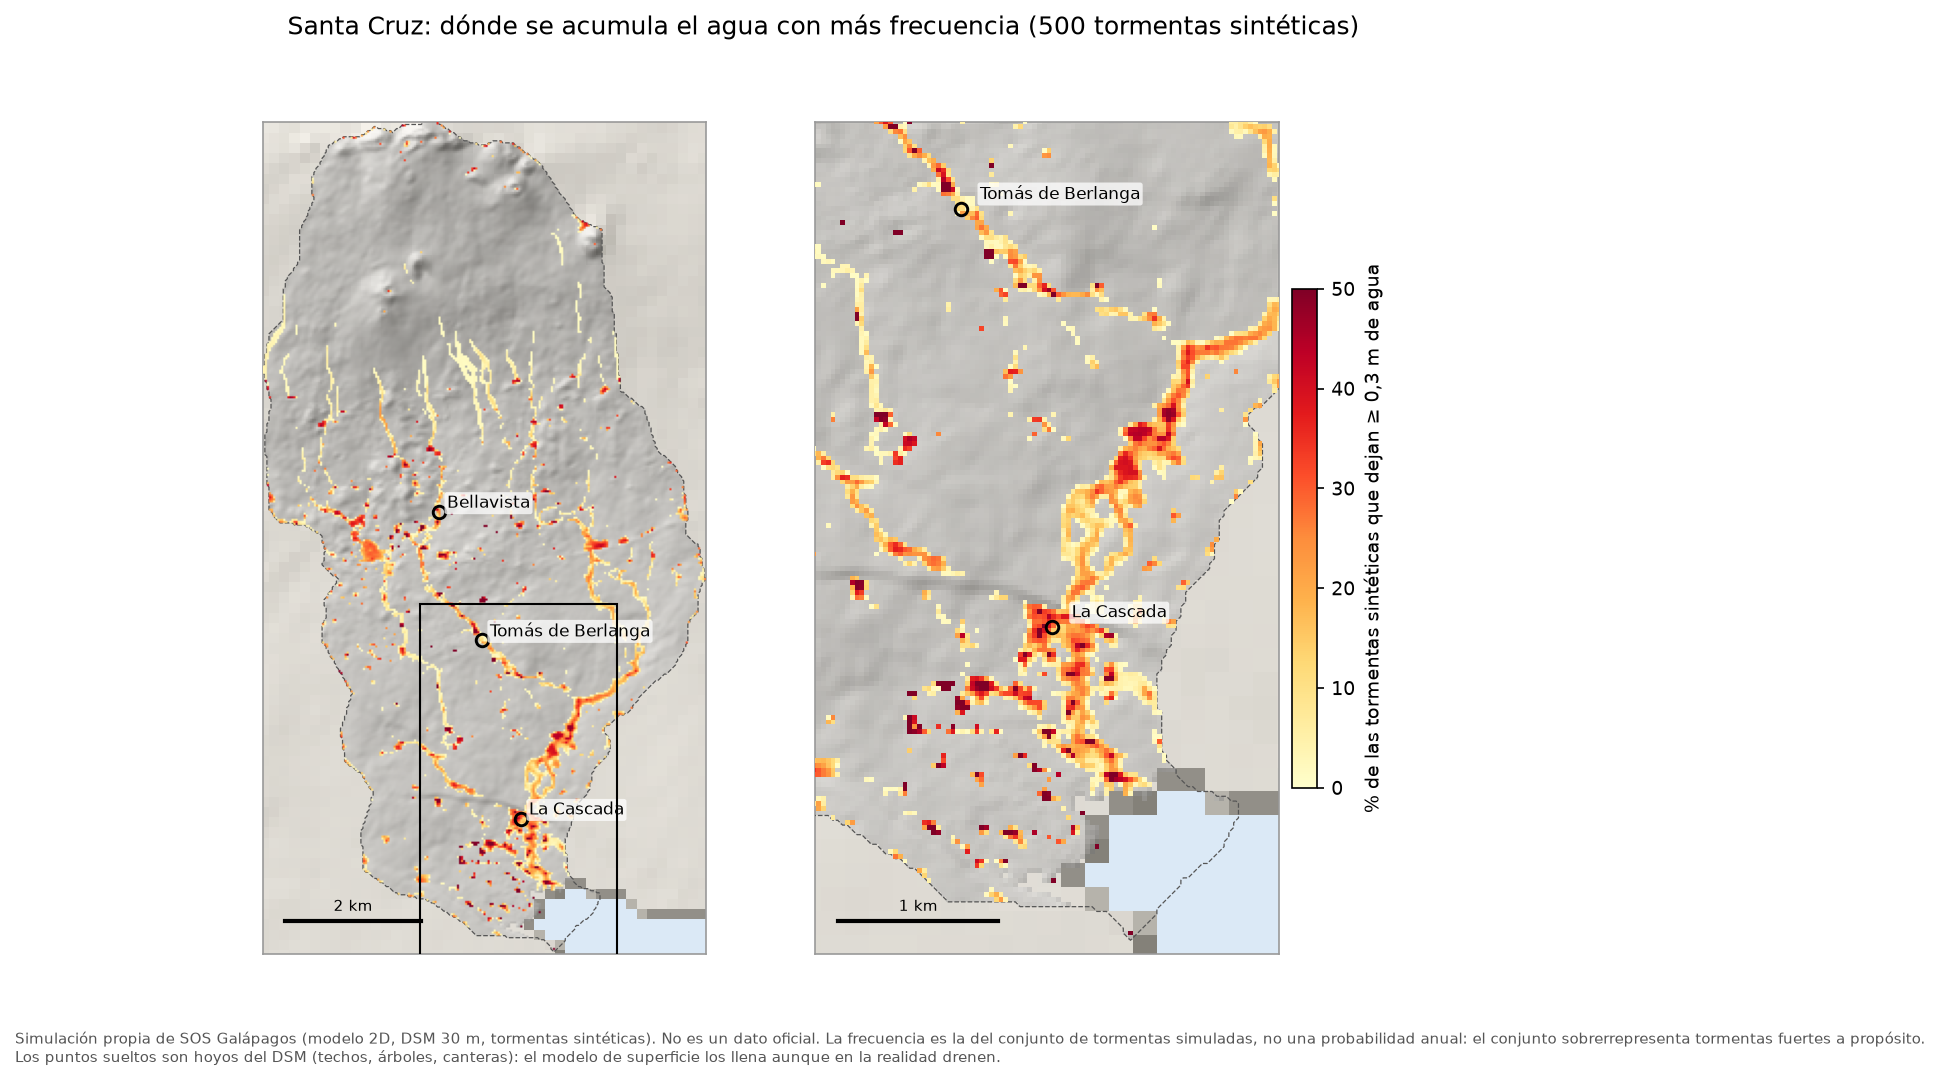
\includegraphics[width=0.92\linewidth]{frecuencia_santa-cruz.png}
  \caption{Fracción de las 500 tormentas sintéticas con calado $\geq 0,3$~m en cada celda de 30~m (Santa Cruz). Es una frecuencia dentro del conjunto sintético, no una probabilidad anual.}
  \label{fig:frecuencia}
\end{figure}

\subsection{Sensibilidad de los umbrales}
Si solo se mira el conjunto sintético, el modelo \enquote{preferiría} umbrales más altos. En La Cascada, 52,5\,/\,75\,/\,190~mm detectarían el 92\,\% de las inundaciones con un 10\,\% de falsas alarmas. Pero la lluvia medida el 30-oct cuenta otra historia (tabla~\ref{tab:umbrales}, figura~\ref{fig:compromiso}). Con la v0.2, el \alto{} se habría dado a las 15:50. Con umbrales un 10\,\% más altos, a las 19:00, y con un 35\,\% más, a las 20:30. El modelo sitúa la llegada del agua al centro del barrio a las 20:55.

La v0.2 está, por tanto, en el borde: una pequeña subida retrasa tres horas el aviso del único evento real disponible. No se conoce la hora real de entrada del agua, así que estos resultados \textbf{no justifican modificar los umbrales} hasta contrastarlos con inundaciones históricas fechadas.

\begin{table}[ht]
  \centering\small
  \caption{Hora a la que se habría dado el \alto{} el 30-oct-2026 en La Cascada según el escalado de los umbrales (lluvia medida por la red IERSE-WSN).}
  \label{tab:umbrales}
  \begin{tabular}{lcc}
    \toprule
    Umbrales de \alto{} (1~h\,/\,3~h\,/\,24~h) & Hora del aviso & Anticipación frente a la llegada modelada (20:55) \\
    \midrule
    v0.2: 30\,/\,60\,/\,100~mm & 15:50 & 5~h~05~min \\
    $\times$\,1,10: 33\,/\,66\,/\,110~mm & 19:00 & 1~h~55~min \\
    $\times$\,1,35: 40\,/\,81\,/\,135~mm & 20:30 & 25~min \\
    \bottomrule
  \end{tabular}
\end{table}

\begin{figure}[t]
  \centering
  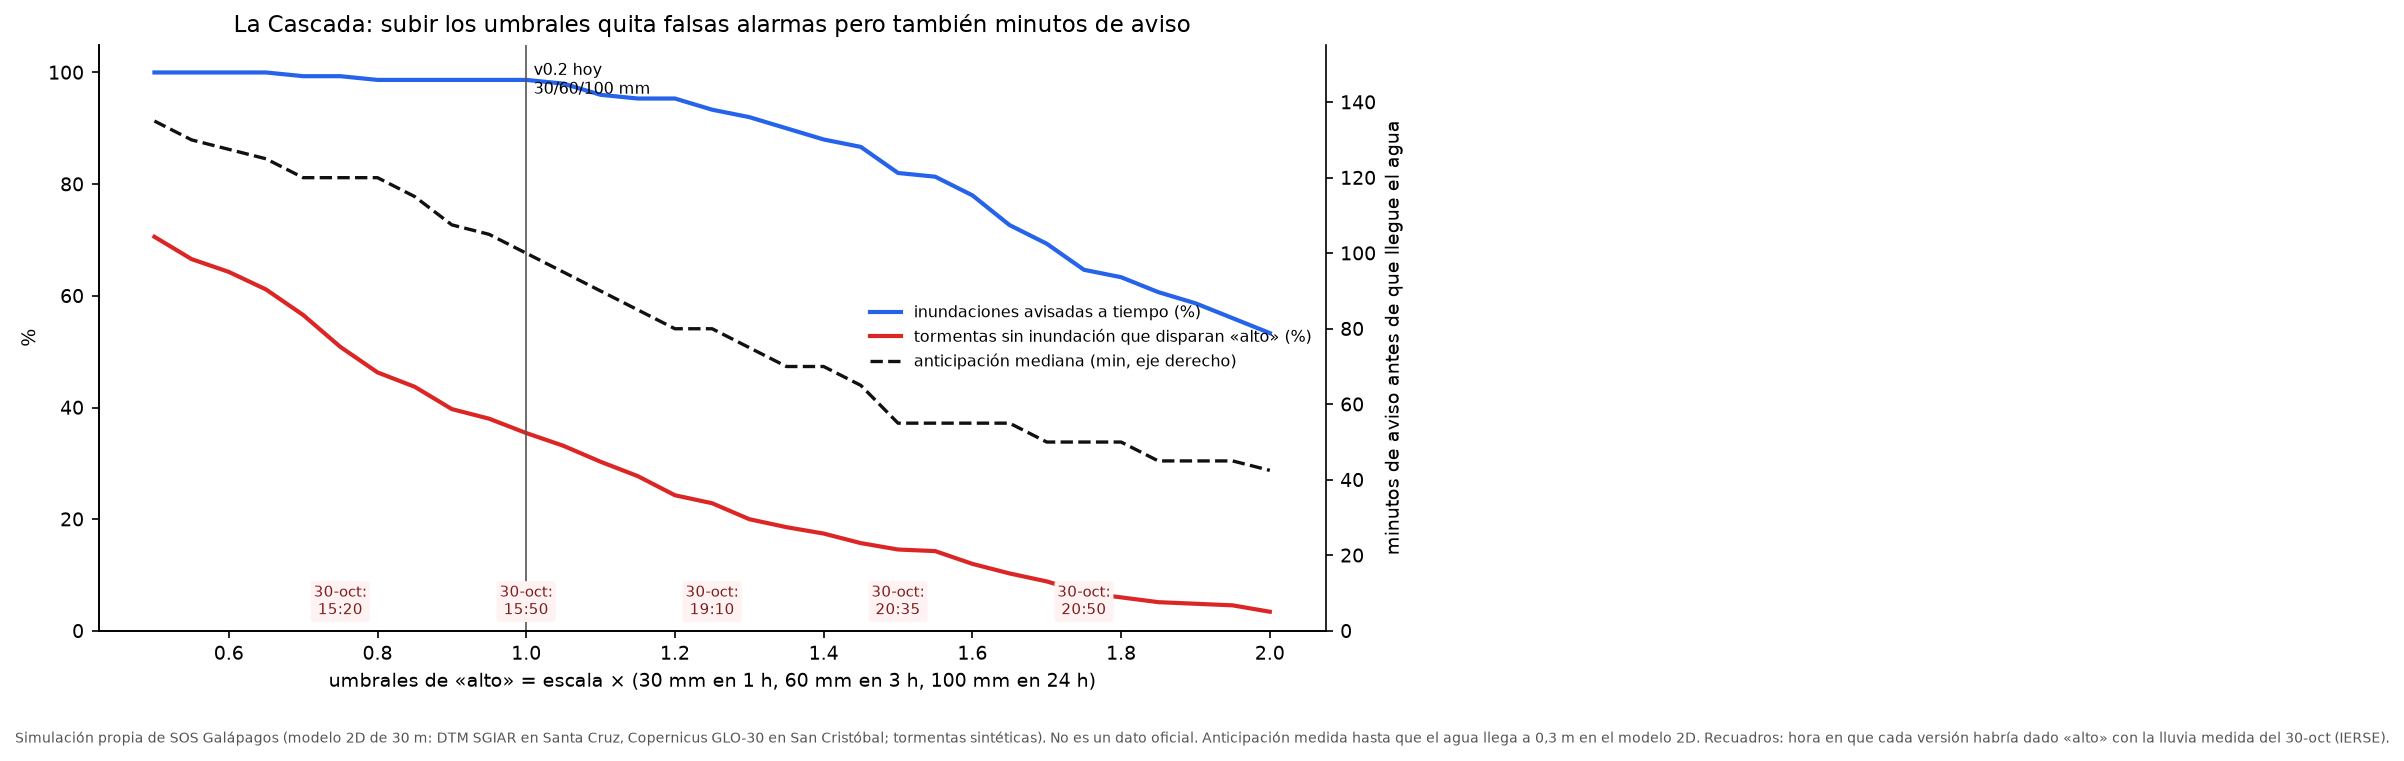
\includegraphics[width=\linewidth]{compromiso_santa-cruz_la_cascada.png}
  \caption{Compromiso entre detección, falsas alarmas y anticipación al escalar los umbrales de \alto{} en La Cascada, con la hora de aviso del 30-oct superpuesta.}
  \label{fig:compromiso}
\end{figure}

\subsection{Qué pluviómetro anticipa mejor}
En La Cascada todas las estaciones actuales discriminan bien (tabla~\ref{tab:auc}); la mejor es Los Guayabillos (AUC 0,94). El mejor sitio nuevo está en la cuenca media ($-90,3112$; $-0,7015$; ${\approx}\,157$~m), con AUC 0,96 (figura~\ref{fig:pluviometros}). Un pluviómetro ahí subiría la detección de la regla del 98\,\% al 100\,\%. Añadir Cerro Crocker también llega al 100\,\%, pero eleva las falsas alarmas del conjunto al 48\,\%.

Hay dos casos con poca capacidad de anticipación:
\begin{itemize}
  \item \textbf{Bellavista:} ninguna estación supera 0,78. Se inunda con chubascos locales que la red no ve.
  \item \textbf{San Cristóbal:} las estaciones altas del GSC (0,61--0,64) anticipan \emph{peor} que la costera del INAMHI (0,79). El Progreso no lo anticipa ningún pluviómetro ($\leq 0,65$): se encharca en depresiones con lluvia local dentro de la hora. Ahí es más útil un sensor de nivel.
\end{itemize}

\begin{table}[ht]
  \centering\small
  \caption{Capacidad de anticipación de cada pluviómetro actual (AUC de la lluvia en las 3~h previas a la llegada del agua) en La Cascada.}
  \label{tab:auc}
  \begin{tabular}{lccccccc}
    \toprule
    & \makecell{Los\\Guayabillos} & \makecell{INAMHI\\P. Ayora} & Erna & \makecell{Punta\\Estrada} & \makecell{Cerro\\Crocker} & \makecell{Santa\\Rosa} & \makecell{Sitio\\nuevo} \\
    \midrule
    AUC & 0,94 & 0,93 & 0,92 & 0,92 & 0,90 & 0,88 & 0,96 \\
    \bottomrule
  \end{tabular}
\end{table}

\begin{figure}[t]
  \centering
  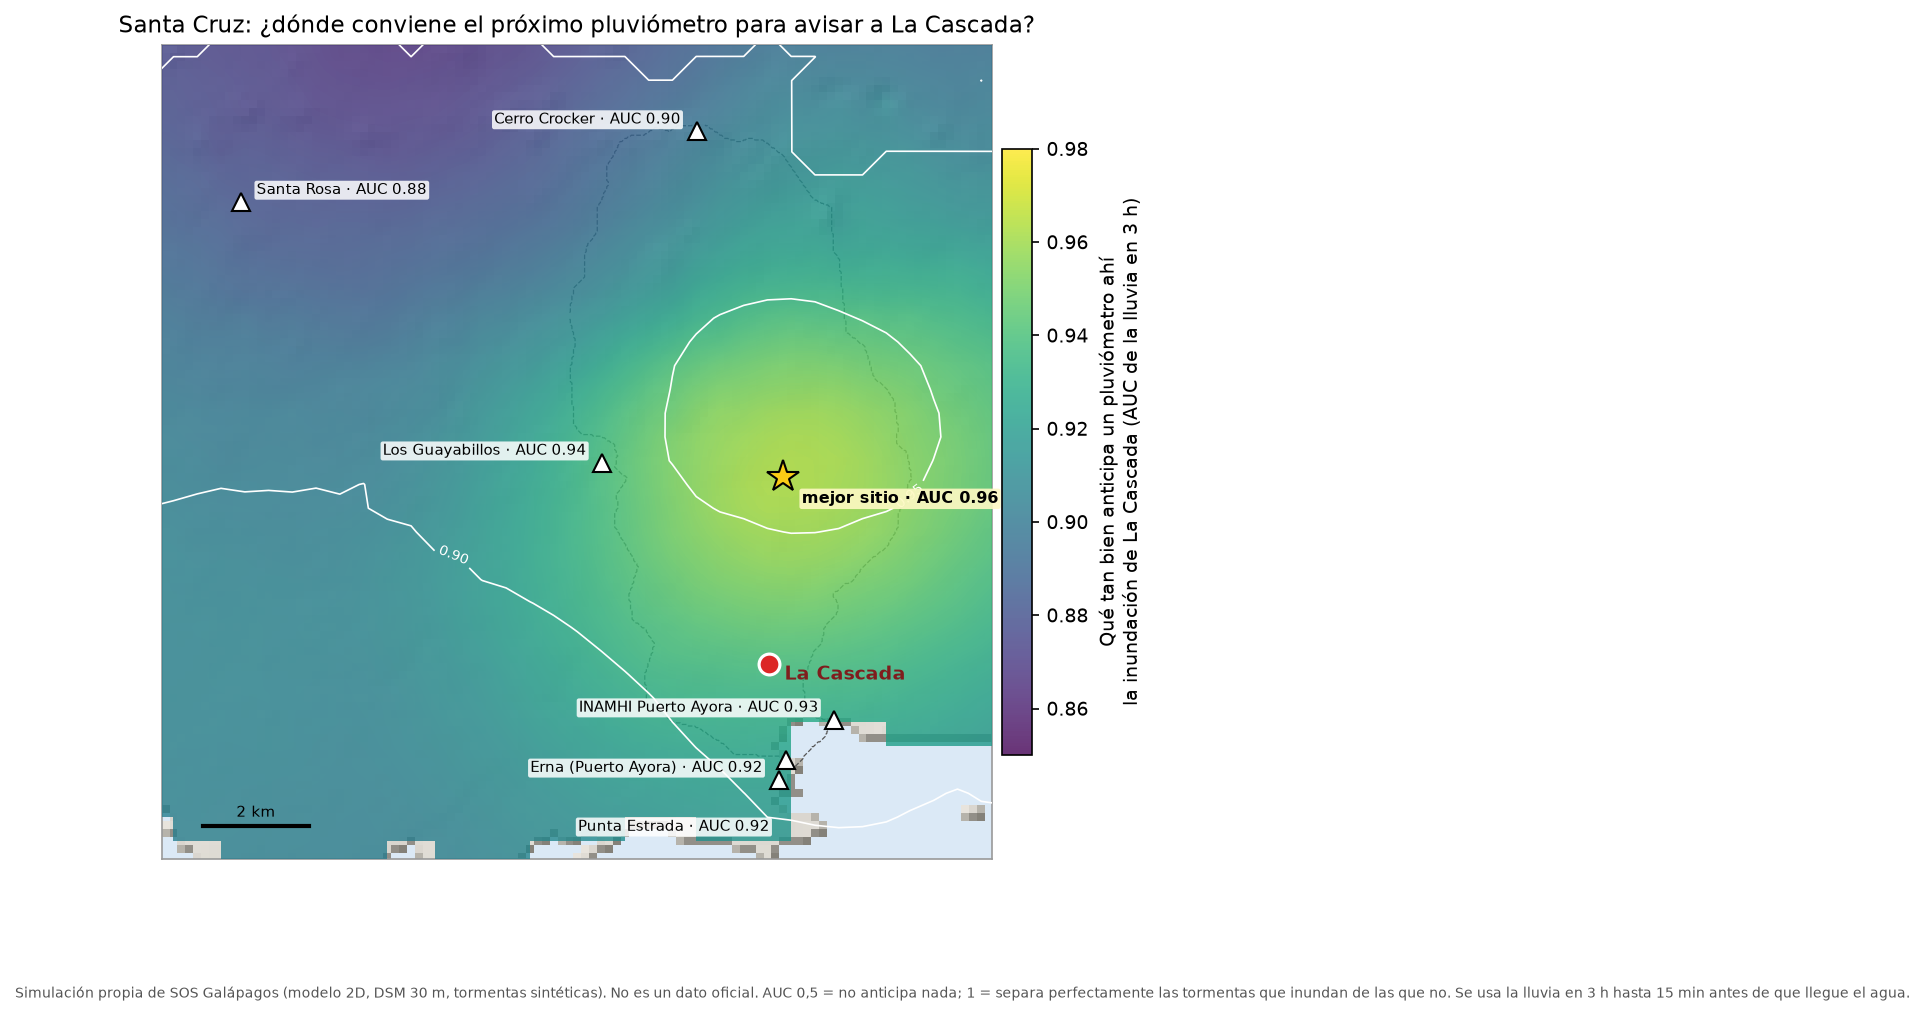
\includegraphics[width=0.92\linewidth]{pluviometros_santa-cruz_la_cascada.png}
  \caption{Capacidad de anticipación (AUC) de la lluvia acumulada en 3~h en cada celda para La Cascada, con las estaciones actuales y el mejor sitio para un pluviómetro nuevo.}
  \label{fig:pluviometros}
\end{figure}

\subsection{Curvas IDF provisionales}
Las razones horarias de GAR van de 0,31 a 0,39 para 1~h. Son algo mayores que las medidas por el IERSE en los días de 40~mm o más (mediana 0,27, rango 0,16--0,47) y coherentes con el 30-oct (0,30--0,36). La tabla~\ref{tab:idf} y las figuras~\ref{fig:idf} y~\ref{fig:metodo} resumen las curvas y el método.

El umbral \alto{} de 30~mm en 1~h equivale a una lluvia de ${\approx}\,2$ años en Los Guayabillos y de ${\approx}\,4$ años en la costa. La GEV tiene una cola más pesada ($\xi \approx 0,2$) y da hasta un 45\,\% más que la Gumbel a 100 años.

\begin{table}[ht]
  \centering\small
  \caption{Láminas de las curvas IDF provisionales (Gumbel). Entre corchetes, el intervalo de confianza del 90\,\% por \emph{bootstrap}.}
  \label{tab:idf}
  \begin{tabularx}{\linewidth}{>{\raggedright\arraybackslash}Xccccc}
    \toprule
    Pluviómetro & \makecell{1~h,\\10 años} & \makecell{3~h,\\10 años} & \makecell{24~h,\\10 años} & \makecell{1~h,\\100 años} & \makecell{24~h,\\100 años} \\
    \midrule
    INAMHI Puerto Ayora (costa) & 41~mm [34--48] & 67~mm & 150~mm & 69~mm & 250~mm \\
    Los Guayabillos (178~m) & 57~mm [43--77] & 95~mm & 164~mm & 92~mm & 265~mm \\
    INAMHI Puerto Baquerizo (curva prestada) & 44~mm & 85~mm & 150~mm & 73~mm & 250~mm \\
    \bottomrule
  \end{tabularx}
\end{table}

\begin{figure}[t]
  \centering
  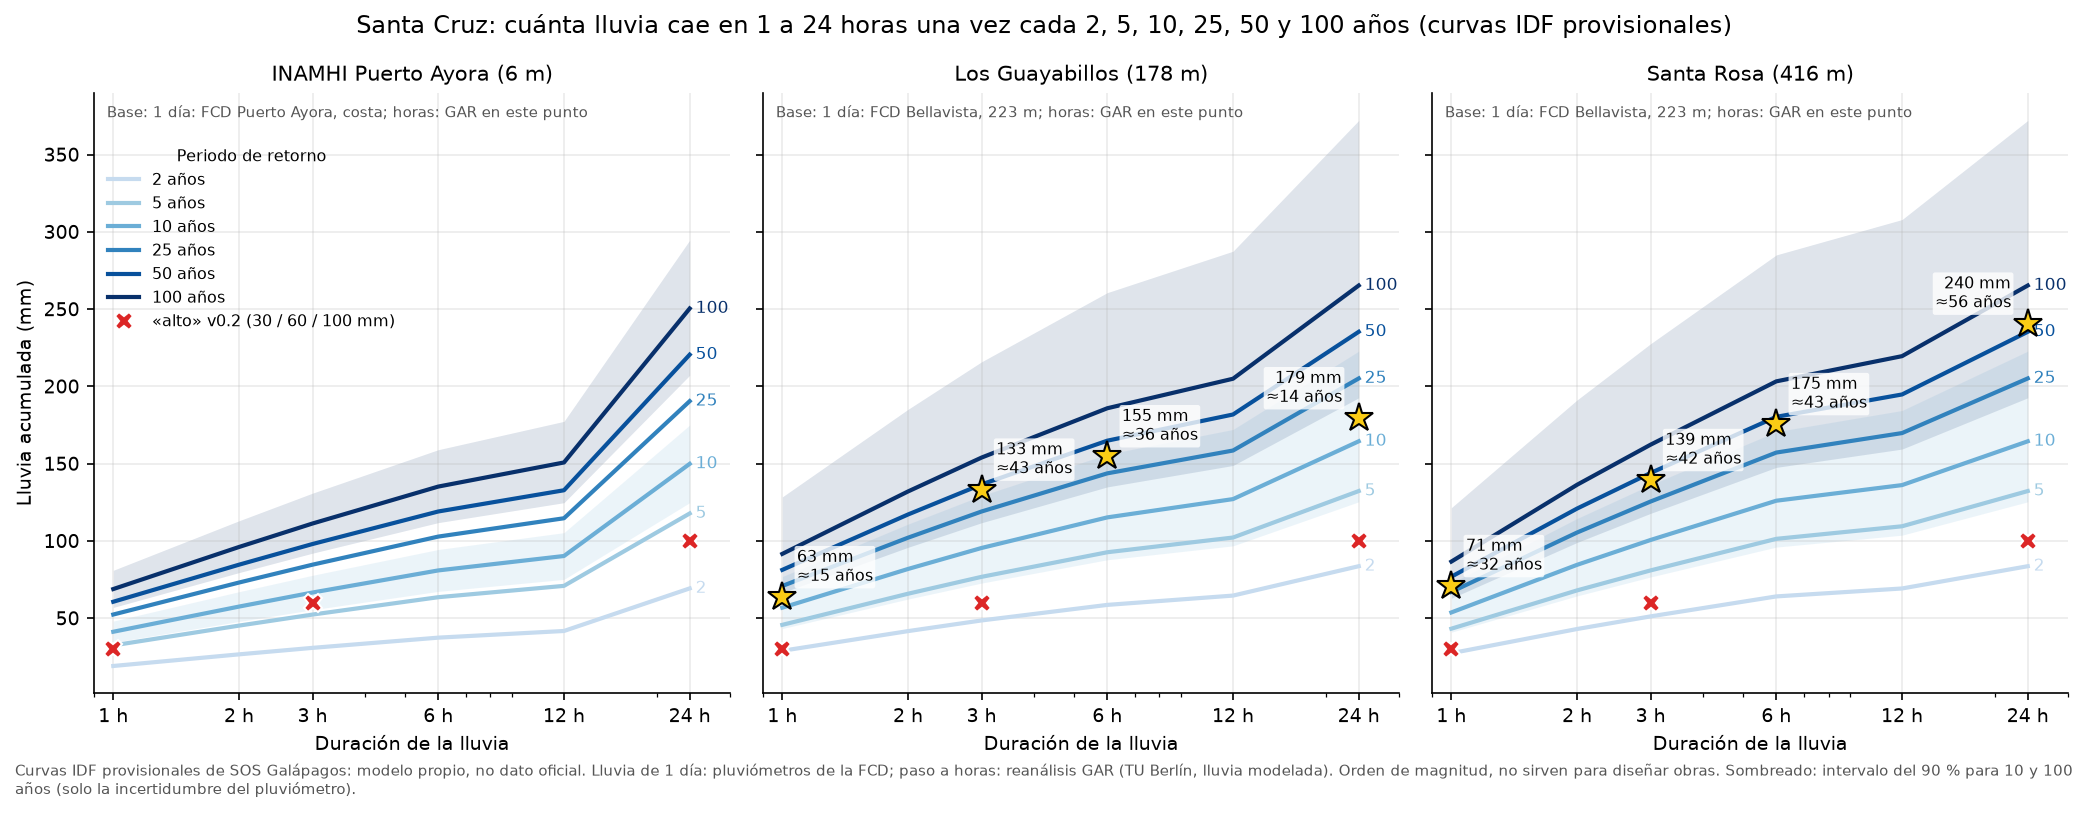
\includegraphics[width=\linewidth]{idf_santa-cruz.png}
  \caption{Curvas IDF provisionales de Santa Cruz para periodos de retorno de 2 a 100 años, con el 30-oct-2026 medido en Los Guayabillos y Santa Rosa.}
  \label{fig:idf}
\end{figure}

\begin{figure}[t]
  \centering
  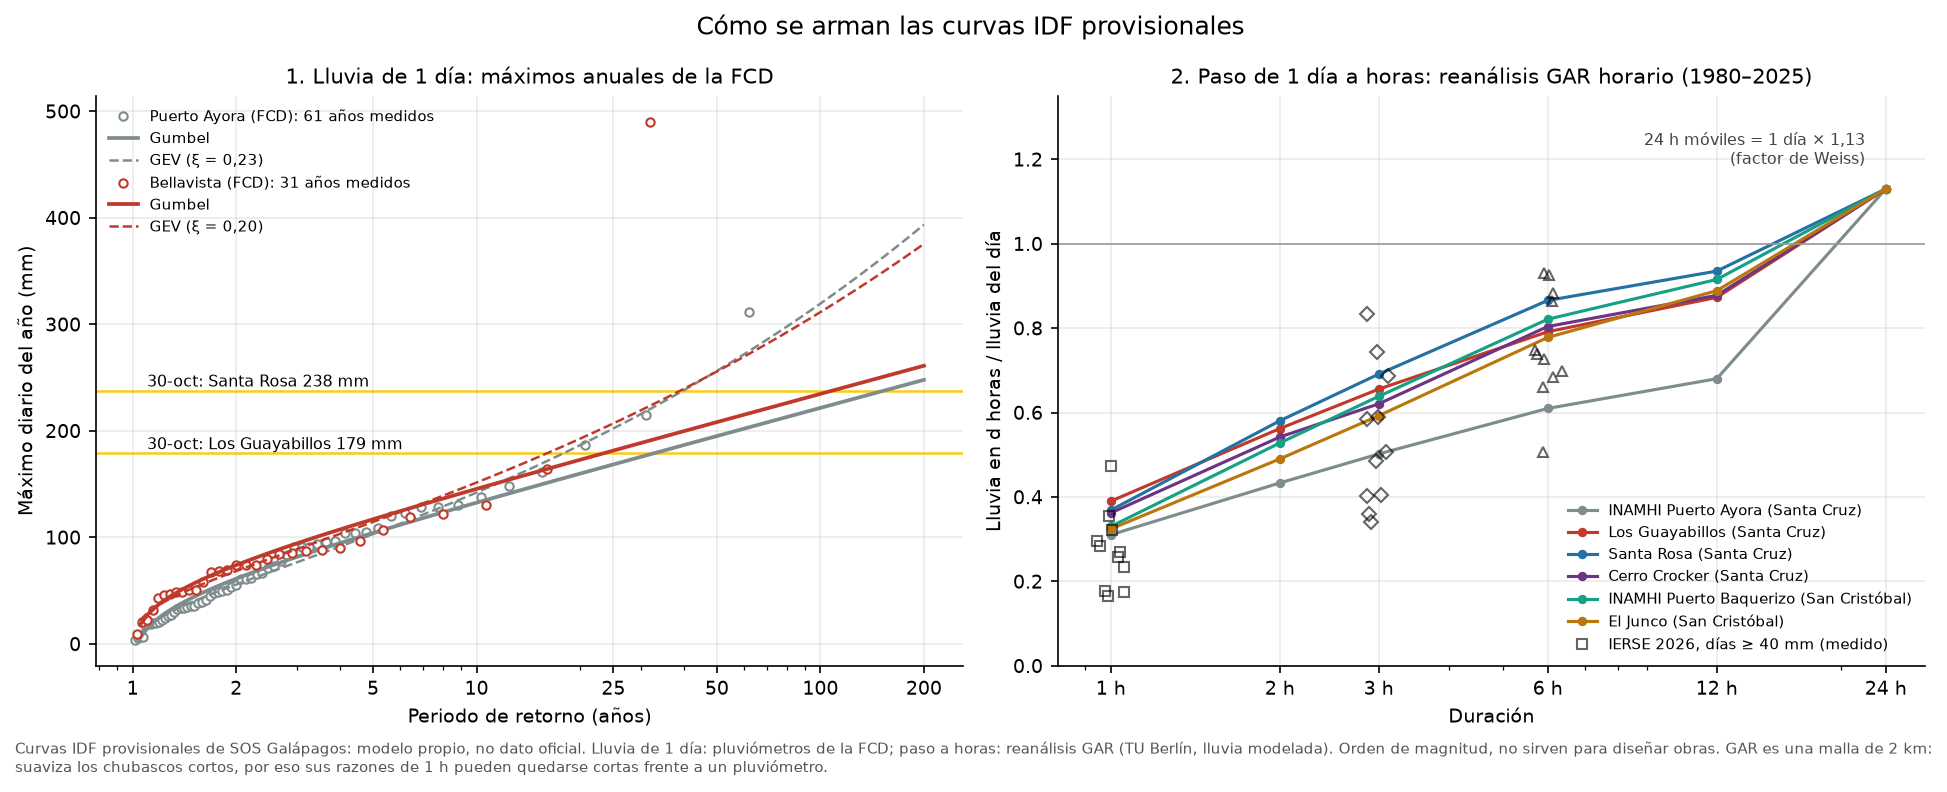
\includegraphics[width=\linewidth]{idf_metodo.png}
  \caption{Método. Izquierda: ajuste de los máximos anuales de un día de la FCD (Gumbel y GEV). Derecha: razones horarias de GAR contrastadas con la lluvia medida cada 5~min (IERSE) y factor de Weiss para 24~h móviles.}
  \label{fig:metodo}
\end{figure}

\subsection{El 30-oct-2026 en la escala de años}
Con la Gumbel, el 30-oct fue una lluvia de unos 15 a 55 años (tabla~\ref{tab:30oct}). Fue más rara en 3--6~h que en 1~h o en el día. Con la GEV los periodos bajan a 11--27 años.

El estudio anterior de Santa Cruz estimó unos 23 años en 24~h. La cifra de aquí es más baja porque se compara con 24~h móviles y no con el día de lectura fija.

\begin{table}[ht]
  \centering\small
  \caption{Periodo de retorno (Gumbel; entre paréntesis, GEV) de la lluvia medida el 30-oct-2026.}
  \label{tab:30oct}
  \begin{tabular}{lcccc}
    \toprule
    Estación & 1~h & 3~h & 6~h & 24~h \\
    \midrule
    Los Guayabillos & \makecell{63~mm\\15 (12) años} & \makecell{133~mm\\43 (23) años} & \makecell{155~mm\\36 (21) años} & \makecell{179~mm\\14 (11) años} \\
    \addlinespace
    Santa Rosa & \makecell{71~mm\\32 (20) años} & \makecell{139~mm\\42 (23) años} & \makecell{175~mm\\43 (23) años} & \makecell{240~mm\\56 (27) años} \\
    \bottomrule
  \end{tabular}
\end{table}

\subsection{Frecuencia anual de inundación y de alertas}\label{sec:res-frecuencia}
La tabla~\ref{tab:anual} combina las curvas de fragilidad (figura~\ref{fig:fragilidad}) con la frecuencia de cada lluvia. Las zonas que más se inundarían son Barrio Frío (${\approx}\,1$ vez cada 8 años) y La Cascada (${\approx}\,1$ vez cada 12 años). La regla v0.2 daría \alto{} una vez cada 1,6--1,9 años en cada zona. En casi todas esas ocasiones no habría inundación, lo que equivale a unas 0,4--0,6 falsas alarmas por año y zona. Es el costo de avisar casi todas las inundaciones. La figura~\ref{fig:mapa} muestra dónde se acumula el agua según el periodo de retorno de la lluvia.

\begin{table}[ht]
  \centering\small
  \caption{Frecuencia anual estimada de inundación (calado $\geq 0,3$~m) y del nivel \alto{} de la regla v0.2. $T_{50}$ = periodo de retorno de la lluvia con el que la zona se inunda la mitad de las veces.}
  \label{tab:anual}
  \begin{tabularx}{\linewidth}{>{\raggedright\arraybackslash}Xcccc}
    \toprule
    Zona & $T_{50}$ & \makecell{Inundación\\${\approx}\,1$ vez cada} & \makecell{\alto{}\\${\approx}\,1$ vez cada} & \makecell{Falsas alarmas\\por año} \\
    \midrule
    La Cascada & 29 años & 12 años & 1,6 años & ${\approx}\,0,6$ \\
    Tomás de Berlanga & $>400$ años & 50 años & 1,6 años & ${\approx}\,0,6$ \\
    Bellavista & 22 años & 10 años & 1,6 años & ${\approx}\,0,5$ \\
    Barrio Frío (desembocadura) & 21 años & 8 años & 1,9 años & ${\approx}\,0,4$ \\
    El Manzanillo & 91 años & 28 años & 1,9 años & ${\approx}\,0,5$ \\
    El Progreso & 94 años & 36 años & 1,9 años & ${\approx}\,0,5$ \\
    \bottomrule
  \end{tabularx}
  \par\vspace{3pt}\raggedright\footnotesize Las cifras de San Cristóbal usan curvas diarias prestadas de Santa Cruz y una pérdida del suelo sin calibrar.
\end{table}

\begin{figure}[t]
  \centering
  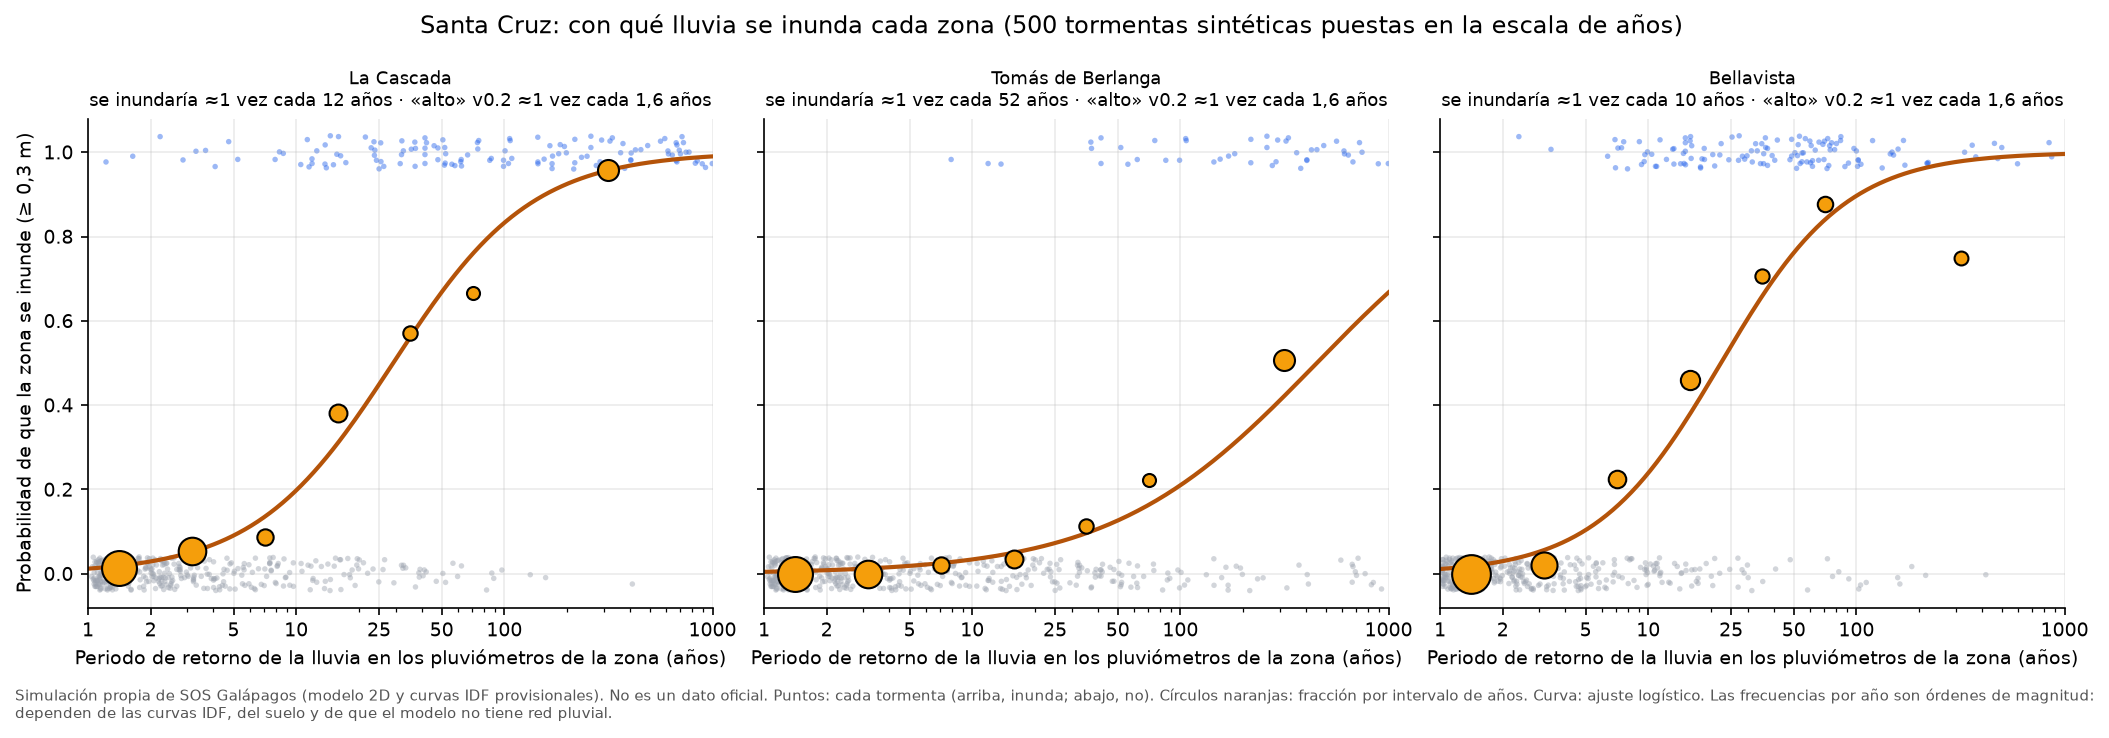
\includegraphics[width=\linewidth]{fragilidad_santa-cruz.png}\\[4pt]
  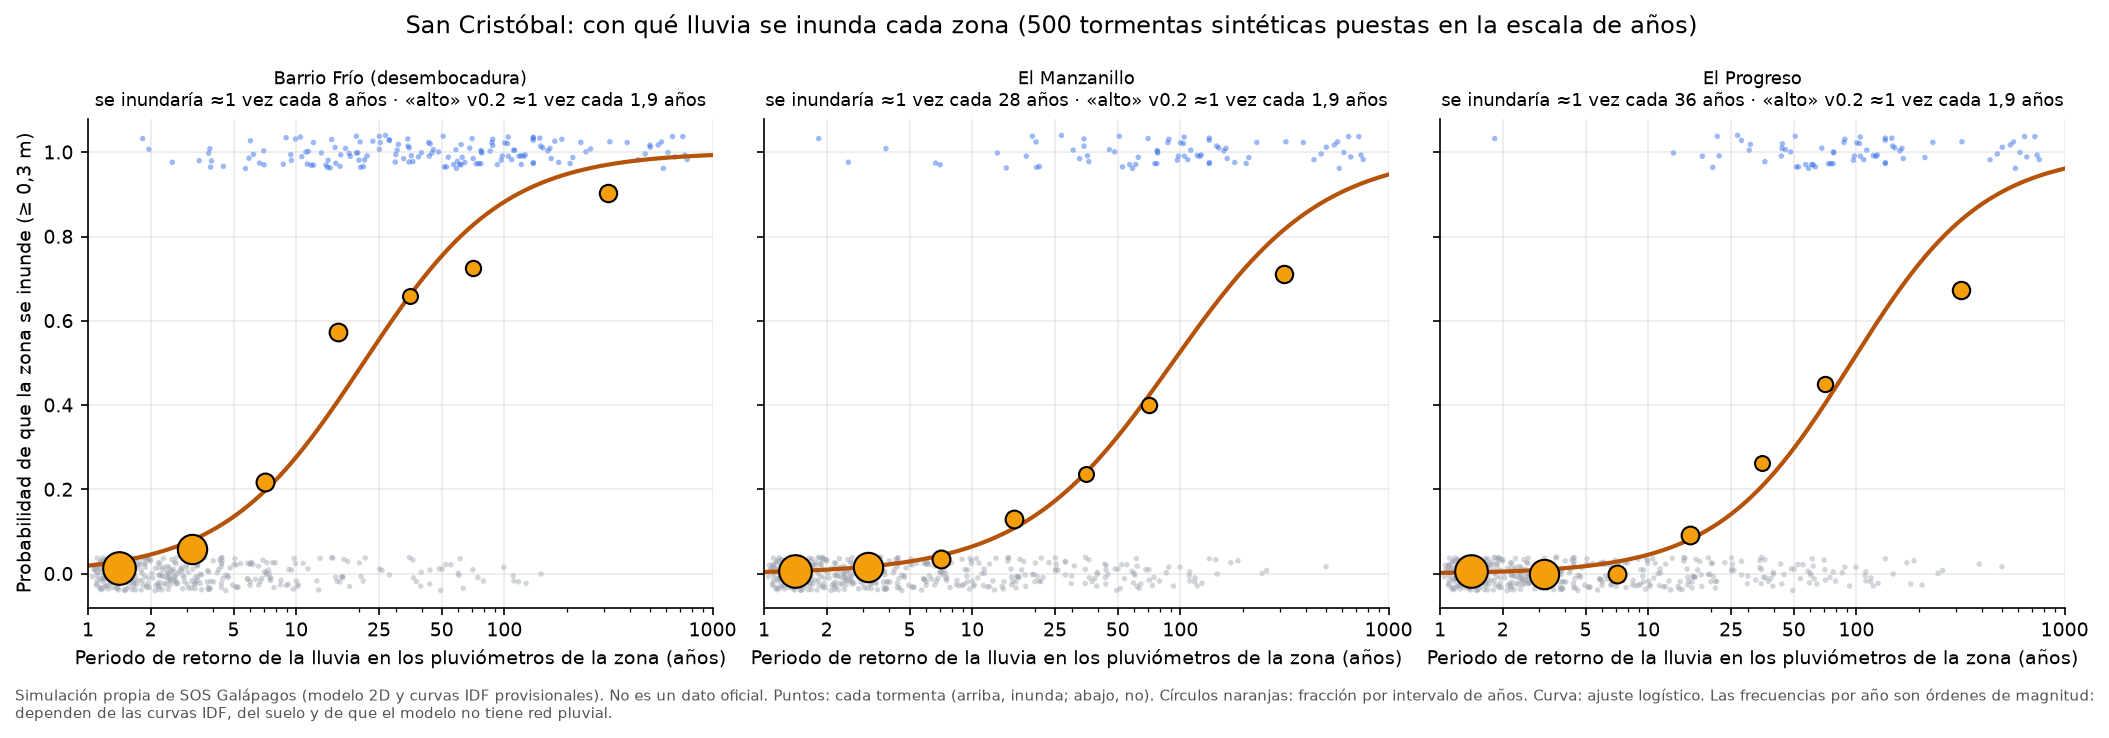
\includegraphics[width=\linewidth]{fragilidad_san-cristobal.png}
  \caption{Curvas de fragilidad: probabilidad de inundación en función del periodo de retorno de la lluvia en los pluviómetros de cada zona (ajuste logístico sobre $\ln T$). Arriba, Santa Cruz; abajo, San Cristóbal, con curvas IDF diarias prestadas de Santa Cruz.}
  \label{fig:fragilidad}
\end{figure}

\begin{figure}[t]
  \centering
  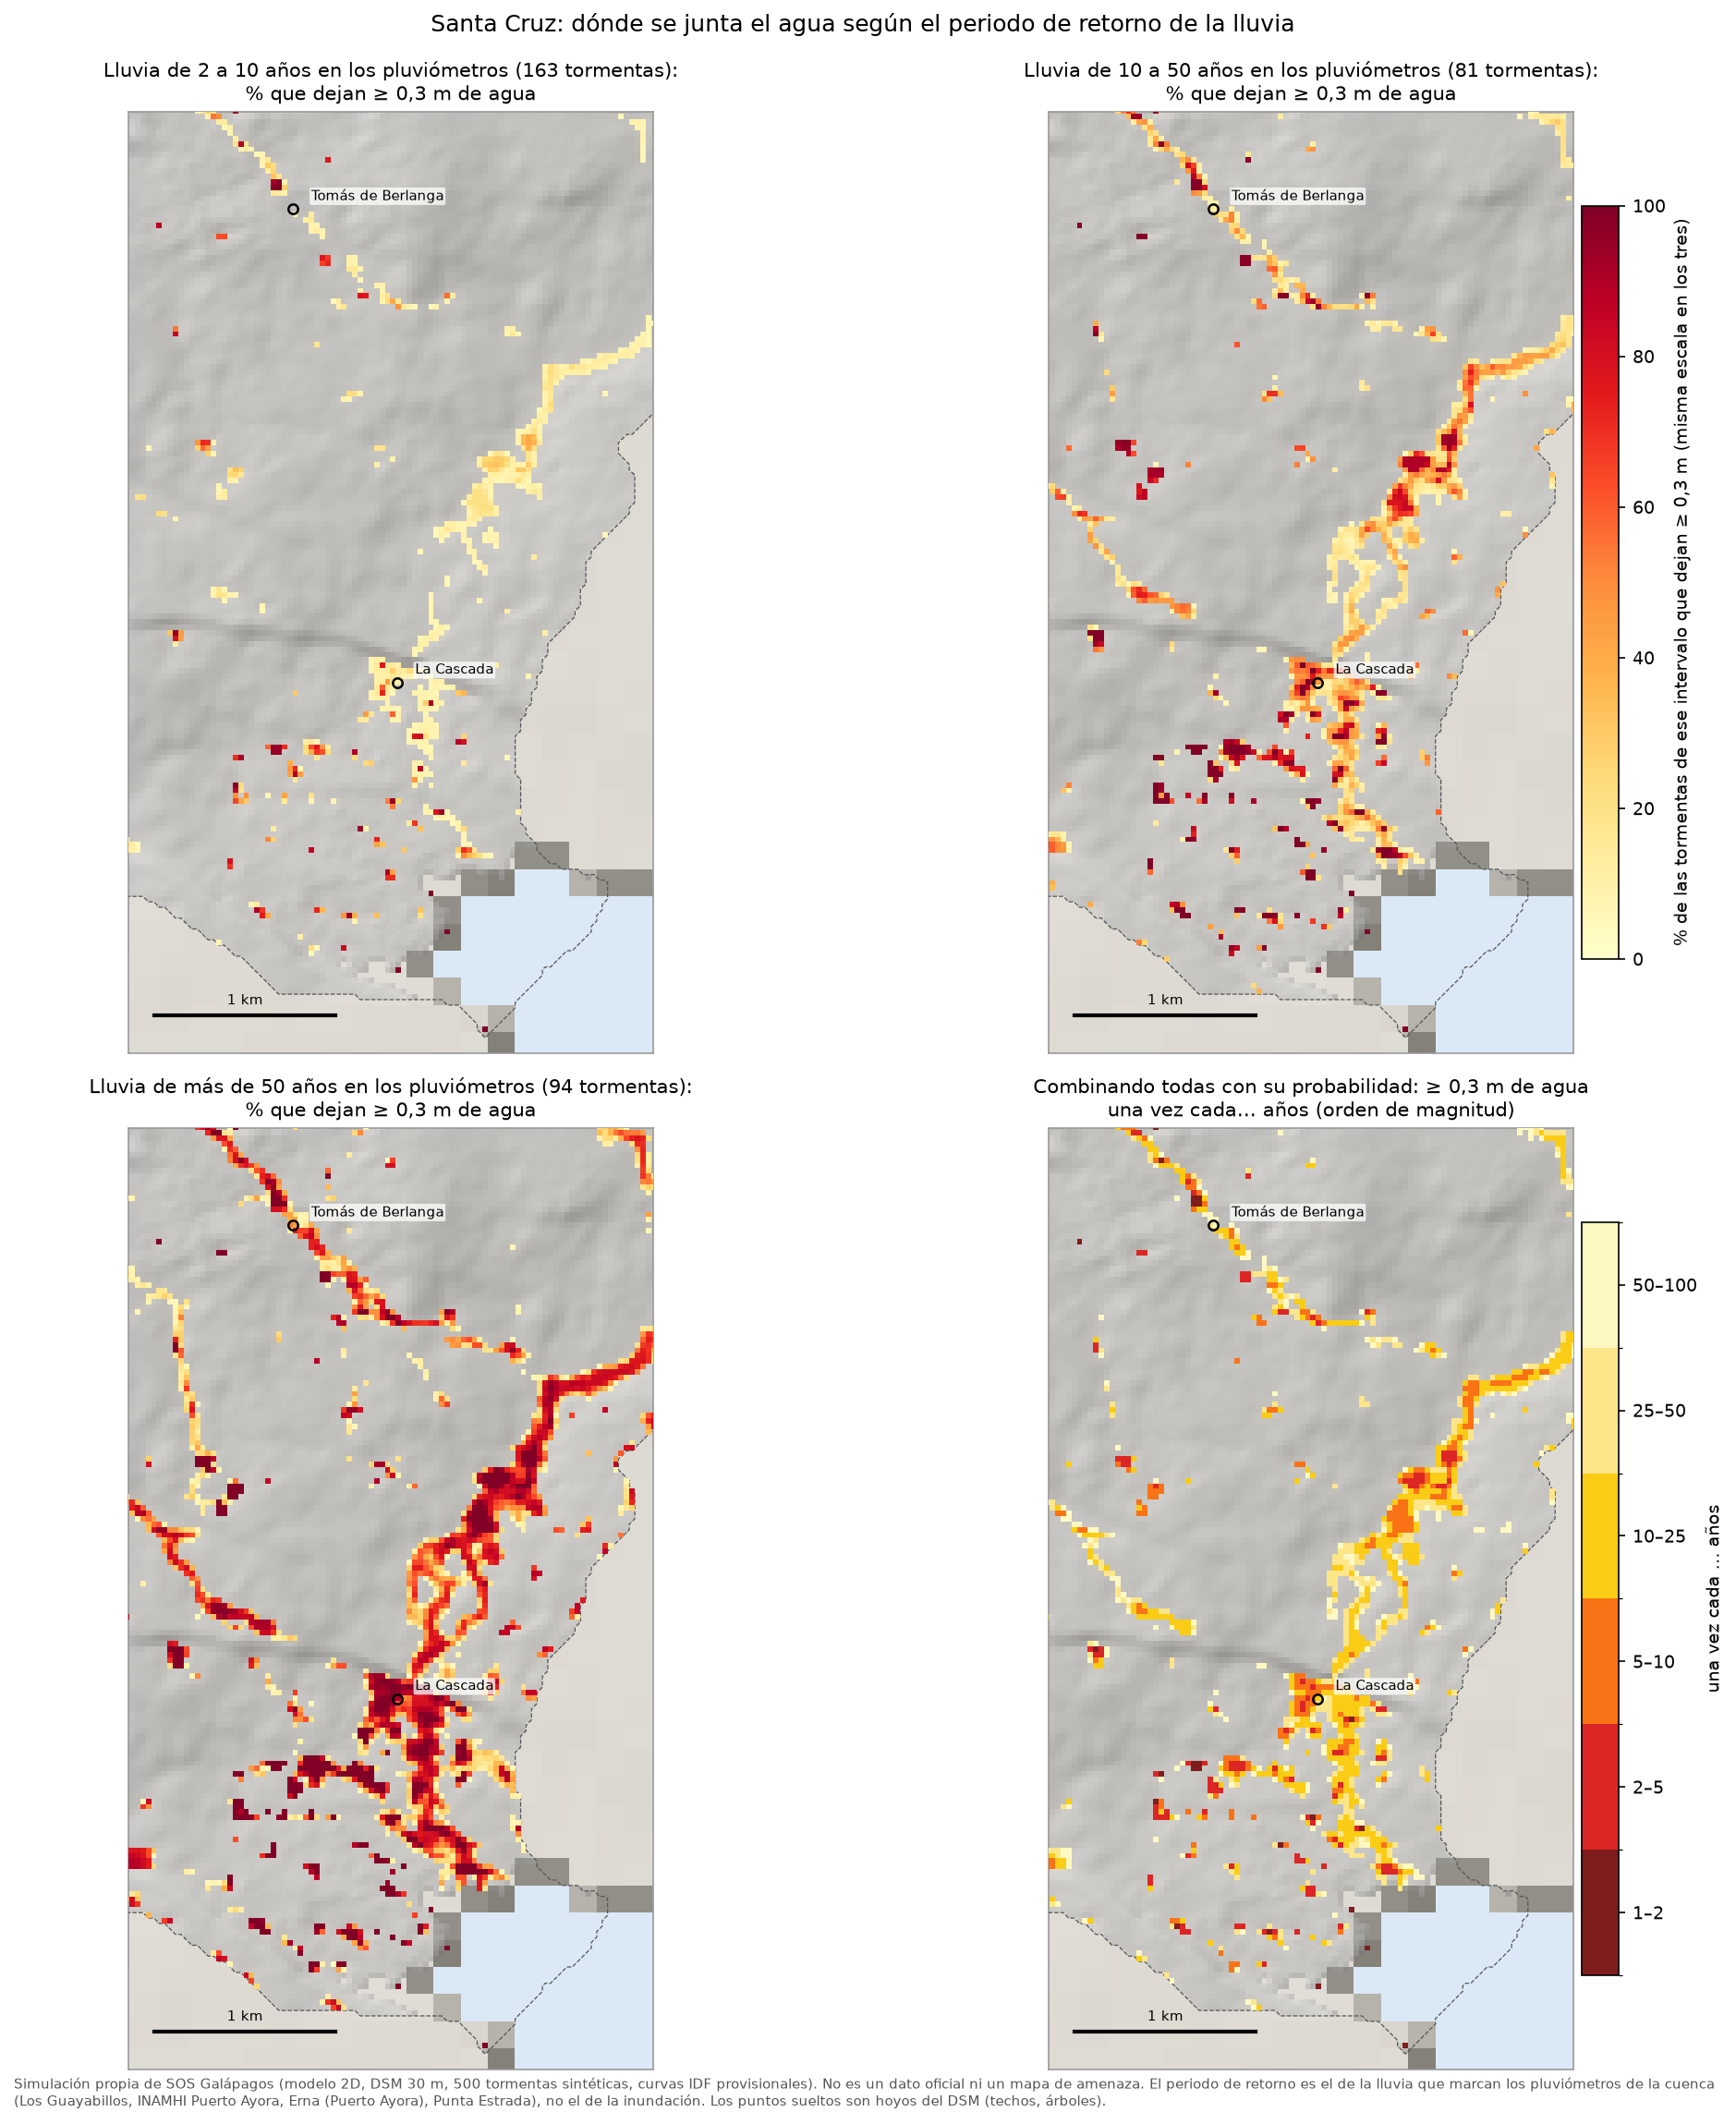
\includegraphics[height=0.6\textheight]{mapa_retorno_santa-cruz.png}
  \caption{Puerto Ayora: fracción de tormentas con calado $\geq 0,3$~m para lluvias de 2--10, 10--50 y $\geq 50$ años, y su combinación en una frecuencia anual (\enquote{una vez cada\ldots\ años}).}
  \label{fig:mapa}
\end{figure}

% =====================================================================
\section{Discusión y limitaciones}

Los resultados son coherentes con mantener la regla v0.2: detecta casi todas las inundaciones modeladas con anticipaciones útiles, y el costo es de una falsa alarma cada dos años por zona. Para una alerta comunitaria ese costo parece aceptable, pero debe comunicarse para no erosionar la confianza.

La mejora con más rendimiento es un pluviómetro en la cuenca media de La Cascada. En El Progreso y Bellavista conviene complementar la lluvia con sensores de nivel, porque los pluviómetros no anticipan lo que pasa allí. Las principales limitaciones son estas:
\begin{itemize}
  \item \textbf{Una sola serie medida por isla, y prestada en San Cristóbal.} La cola de 50--100 años sale de 31--61 años de datos. El dato de Bellavista de marzo de 2008 (490~mm) está en duda y pesa en la cola.
  \item \textbf{GAR es lluvia modelada en una malla de 2~km.} Suaviza los chubascos cortos, y las ventanas horarias no cruzan la medianoche UTC.
  \item \textbf{El periodo de retorno es el de la lluvia, no el de la inundación.} Ambos coinciden solo si la respuesta de la cuenca no depende de otros factores, como la humedad antecedente o la forma de la tormenta.
  \item \textbf{Modelo 2D.} El DSM incluye techos y árboles, y no hay red pluvial. La pérdida del suelo no está calibrada en San Cristóbal. Los pluviómetros sintéticos no tienen error, y La Planada no se inunda en el modelo: probablemente es un problema de drenaje urbano.
  \item \textbf{Sin validación histórica.} No hay registro de inundaciones con hora y profundidad con el cual contrastar las frecuencias de la tabla~\ref{tab:anual}.
\end{itemize}

% =====================================================================
\section{Conclusiones y trabajo futuro}
\begin{enumerate}
  \item La regla v0.2 avisa a tiempo el 87--100\,\% de las inundaciones modeladas, con 25~min a 2~h de anticipación. Daría \alto{} una vez cada 1,6--1,9 años por zona.
  \item El 30-oct-2026 fue una lluvia de unos 15 a 55 años según la duración y la estación.
  \item Barrio Frío y La Cascada serían las zonas más expuestas, con inundaciones del orden de una vez por década.
  \item Subir los umbrales un 10\,\% habría retrasado tres horas el aviso del 30-oct. Sin validación histórica, los resultados no justifican modificarlos.
\end{enumerate}

Para pasar de provisional a robusto hacen falta:
\begin{itemize}
  \item el estudio de intensidades del INAMHI (2015) y las series diarias de San Cristóbal (\issue{77}, \issue{78});
  \item la tesis de la USFQ sobre las encañadas (\issue{79});
  \item un registro de inundaciones históricas con fecha, hora, lugar y profundidad (\issue{80});
  \item un pluviómetro en la cuenca media de La Cascada (\issue{19}) y un sensor de nivel en El Progreso (\issue{81});
  \item más años de lluvia medida cada 5 minutos.
\end{itemize}

\section*{Disponibilidad de datos y código}
{\small Todo el procesamiento es reproducible desde el repositorio público \emph{mayait/sosgalapagos-datos}:
\begin{itemize}
  \item \texttt{geodatos/scripts/32\_tormentas\_sinteticas.py} (generador y motor 2D);
  \item \texttt{33\_tormentas\_figuras.py} (figuras);
  \item \texttt{34\_curvas\_idf.py} (curvas IDF y frecuencias anuales).
\end{itemize}
Los resultados tabulados están en \texttt{geodatos/estudios/tormentas/datos/} y \texttt{geodatos/estudios/idf/datos/}. Este informe se compila con \texttt{informes/compilar.sh 2026-02-tormentas-idf}.\par}

\bibliographystyle{sosg}
\bibliography{referencias}

\end{document}
